\documentclass[12pt,a4paper,french,fleqn]{beamer}

\usepackage{tikz}

\begin{document}

\newcommand{\ax}{-3}
\newcommand{\ay}{-3}
\newcommand{\bx}{0}
\newcommand{\by}{-3}
\newcommand{\cx}{2}
\newcommand{\cy}{2}
\newcommand{\dx}{-1}
\newcommand{\dy}{2}




\begin{frame}
    \begin{minipage}[t]{0.65\textwidth}
        \begin{figure}
            \center
            \begin{tikzpicture}[scale=0.8]
                \draw[dotted,blue] (-4,-4) grid (4,4);
                \draw [blue,thick,->] (0,-4)-- (0,4);
                \draw [blue,thick,->] (-4,0)-- (4,0);
            \end{tikzpicture}
        \end{figure}
    \end{minipage}
    \hfil
    \vrule
    \hfil
    \begin{minipage}[t]{0.32\textwidth}
        \underbar{Placer les points :}
        
        \begin{itemize}
            \item A(\ax ; \ay)
            \item B(\bx ; \by)
            \item C(\cx ; \cy)
            \item D(\dx ; \dy)
        \end{itemize}
        Tracer le parallélogramme ABCD et calculer son aire.
    \end{minipage}
\end{frame}


\begin{frame}
    \begin{minipage}[t]{0.65\textwidth}
        \begin{figure}
            \center
            \begin{tikzpicture}[scale=0.8]
                \draw[dotted,blue] (-4,-4) grid (4,4);
                \draw [blue,thick,->] (0,-4)-- (0,4);
                \draw [blue,thick,->] (-4,0)-- (4,0);
                \draw (\ax,\ay)--(\bx,\by)--(\cx,\cy)--(\dx,\dy)--cycle;
            \end{tikzpicture}
        \end{figure}
    \end{minipage}
    \hfil
    \vrule
    \hfil
    \begin{minipage}[t]{0.32\textwidth}
        \underbar{Placer les points :}
        
        \begin{itemize}
            \item A(\ax ; \ay)
            \item B(\bx ; \by)
            \item C(\cx ; \cy)
            \item D(\dx ; \dy)
        \end{itemize}
        Tracer le parallélogramme ABCD et calculer son aire.
    \end{minipage}
\end{frame}

\begin{frame}
        \underbar{Calculer l'aire des parallélogrammes suivants :}
    \begin{figure}
            \center
            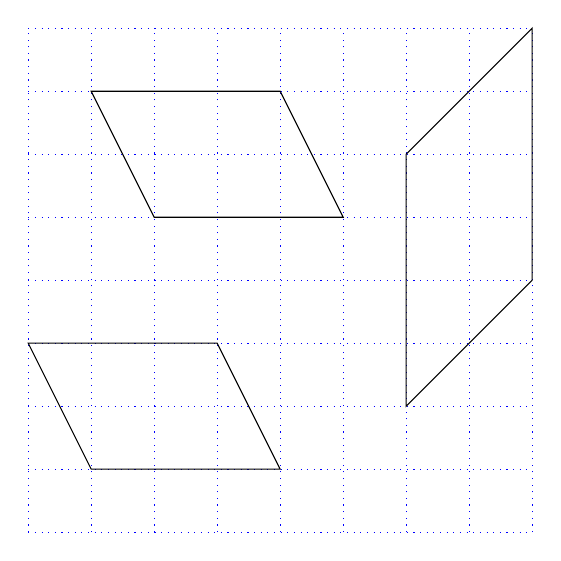
\begin{tikzpicture}[scale=0.8]
                \draw[dotted,blue] (-4,-4) grid (4,4);
                \draw (-3,3)--(0,3)--(1,1)--(-2,1)--cycle ; 
                \draw (4,4)--(4,0)--(2,-2)--(2,2)--cycle ; 
                \draw (-3,-3)--(0,-3)--(-1,-1)--(-4,-1)--cycle ; 
            \end{tikzpicture}
        \end{figure}
\end{frame}

\begin{frame}
        \underbar{Calculer l'aire des parallélogrammes suivants :}
    \begin{figure}
            \center
            \begin{tikzpicture}[scale=0.8]
                \draw[dotted,blue] (-4,-4) grid (4,4);
                \draw (-3,-3)--(0,-3)--(4,3)--(1,3)--cycle ; 
            \end{tikzpicture}
        \end{figure}
\end{frame}

\renewcommand{\ax}{-3}
\renewcommand{\ay}{-3}
\renewcommand{\bx}{-1}
\renewcommand{\by}{-3}
\renewcommand{\cx}{1}
\renewcommand{\cy}{-2}
\renewcommand{\dx}{-1}
\renewcommand{\dy}{-2}

\begin{frame}
        \underbar{Calculer l'aire des parallélogrammes suivants :}
    \begin{figure}
            \center
            \begin{tikzpicture}[scale=0.8]
                \draw[dotted,blue] (-4,-4) grid (4,4);
                \draw (-3,3)--(-1,3)--(1,1)--(-1,1)--cycle ; 
                \draw (4,4)--(4,2)--(2,-2)--(2,0)--cycle ; 
                \draw (\ax,\ay)--(\bx,\by)--(\cx,\cy)--(\dx,\dy)--cycle;
            \end{tikzpicture}
        \end{figure}
\end{frame}
\end{document}
